\documentclass[uplatex, a4paper, 12pt, openany, oneside]{jsbook}
\usepackage[hang,small,bf]{caption}
\usepackage[subrefformat=parens]{subcaption}
\captionsetup{compatibility=false}
% \usepackage{caption}
% \usepackage{subcaption}
\usepackage[ipa]{pxchfon}
\captionsetup[figure]{justification=centering}
\captionsetup[table]{justification=centering}
\usepackage[T1]{fontenc}
\usepackage{amsmath}
\usepackage{enumitem}
\usepackage[dvipdfmx]{graphicx}
\usepackage[dvipdfmx]{color}
\usepackage[dvipdfmx, bookmarks=true, setpagesize=false, hidelinks]{hyperref}
\usepackage{pxjahyper}
\usepackage{thesis}
\usepackage{here}
\usepackage{url}


\thesis{卒 業 論 文}
\title{
  \centering
    \scalebox{1.0}{AIFormulaにおける経路追従ソフトウェアの検討}\\
    \vspace{-0.3zh}
    \scalebox{0.7}{Examination of route-following software in AIFormula}
    \vspace{-0.6zh}
}
\setlength{\textwidth}{\fullwidth}
\setlength{\evensidemargin}{\oddsidemargin}

\date{\today}
\vspace{-15.0zh}
\teacher{林原 靖男 教授}
\vspace{-15.0zh}
\organization{千葉工業大学 先進工学部 未来ロボティクス学科}
\author{21C1135 山下響}
\vspace{-15zh}

\renewcommand{\baselinestretch}{1.2}
\begin{document}

%% Front Matter
\frontmatter{}
%
\chapter{序論}
\label{chap:introduction}
%
%\input{introduction/preface}
%
%!TEX root = ../thesis.tex

\section{背景}
AIFormulaは計測自動制御学会と自動車技術会が主催し, 本田技術研究所がサポートする次世代の人工知能モビリティの競技会で, 正式な競技会は2025年から始まる.
AIFormulaは今後ますます需要が高まるであろう自動化システムの技術者を育てるという点で効果が見込まれる.
AIFormulaではハードウェアの変更もある程度許容されているが, 現時点での開発はソフトウェアが中心となる.
ハードウェアは経路追従するために必要なパーツが全て揃っているが, ソフトウェアはデバイスを駆動するサンプルプログラムが用意されているのみである.
競技という性質上, 経路追従などのソフトウェアは各チームで開発することが必要となる.
その点で, コースを自動で走行するためにはソフトウェアの開発は必須となる.

\subsection{ハードウェアとルール}
AIFormulaでは詳細なルールは検討中であるとのことで, 2025年2月に開催される予定のプレ大会以降に詳細なルールが決定される予定となっている.
Fig.1に2025年のプレ大会で使用されるロボットを示す.
プレ大会では指定されたコースを3周する時間で競われる.
LiDARなどは使用できないなど, いくつかの制約がある.

\begin{figure}[H]
  \centering
 \includegraphics[keepaspectratio, scale=0.6]
      {images/ExteriorViewOfTheMobilityPlatform.png}
 \caption{Exterior view of the mobility platform}
 \label{fig:robot view}
\end{figure}

\subsection{コース}
Fig.2にAIFormulaのコースを示す.
周囲に高い建造物のない平坦なコースである.


\begin{figure}[H]
  \centering
 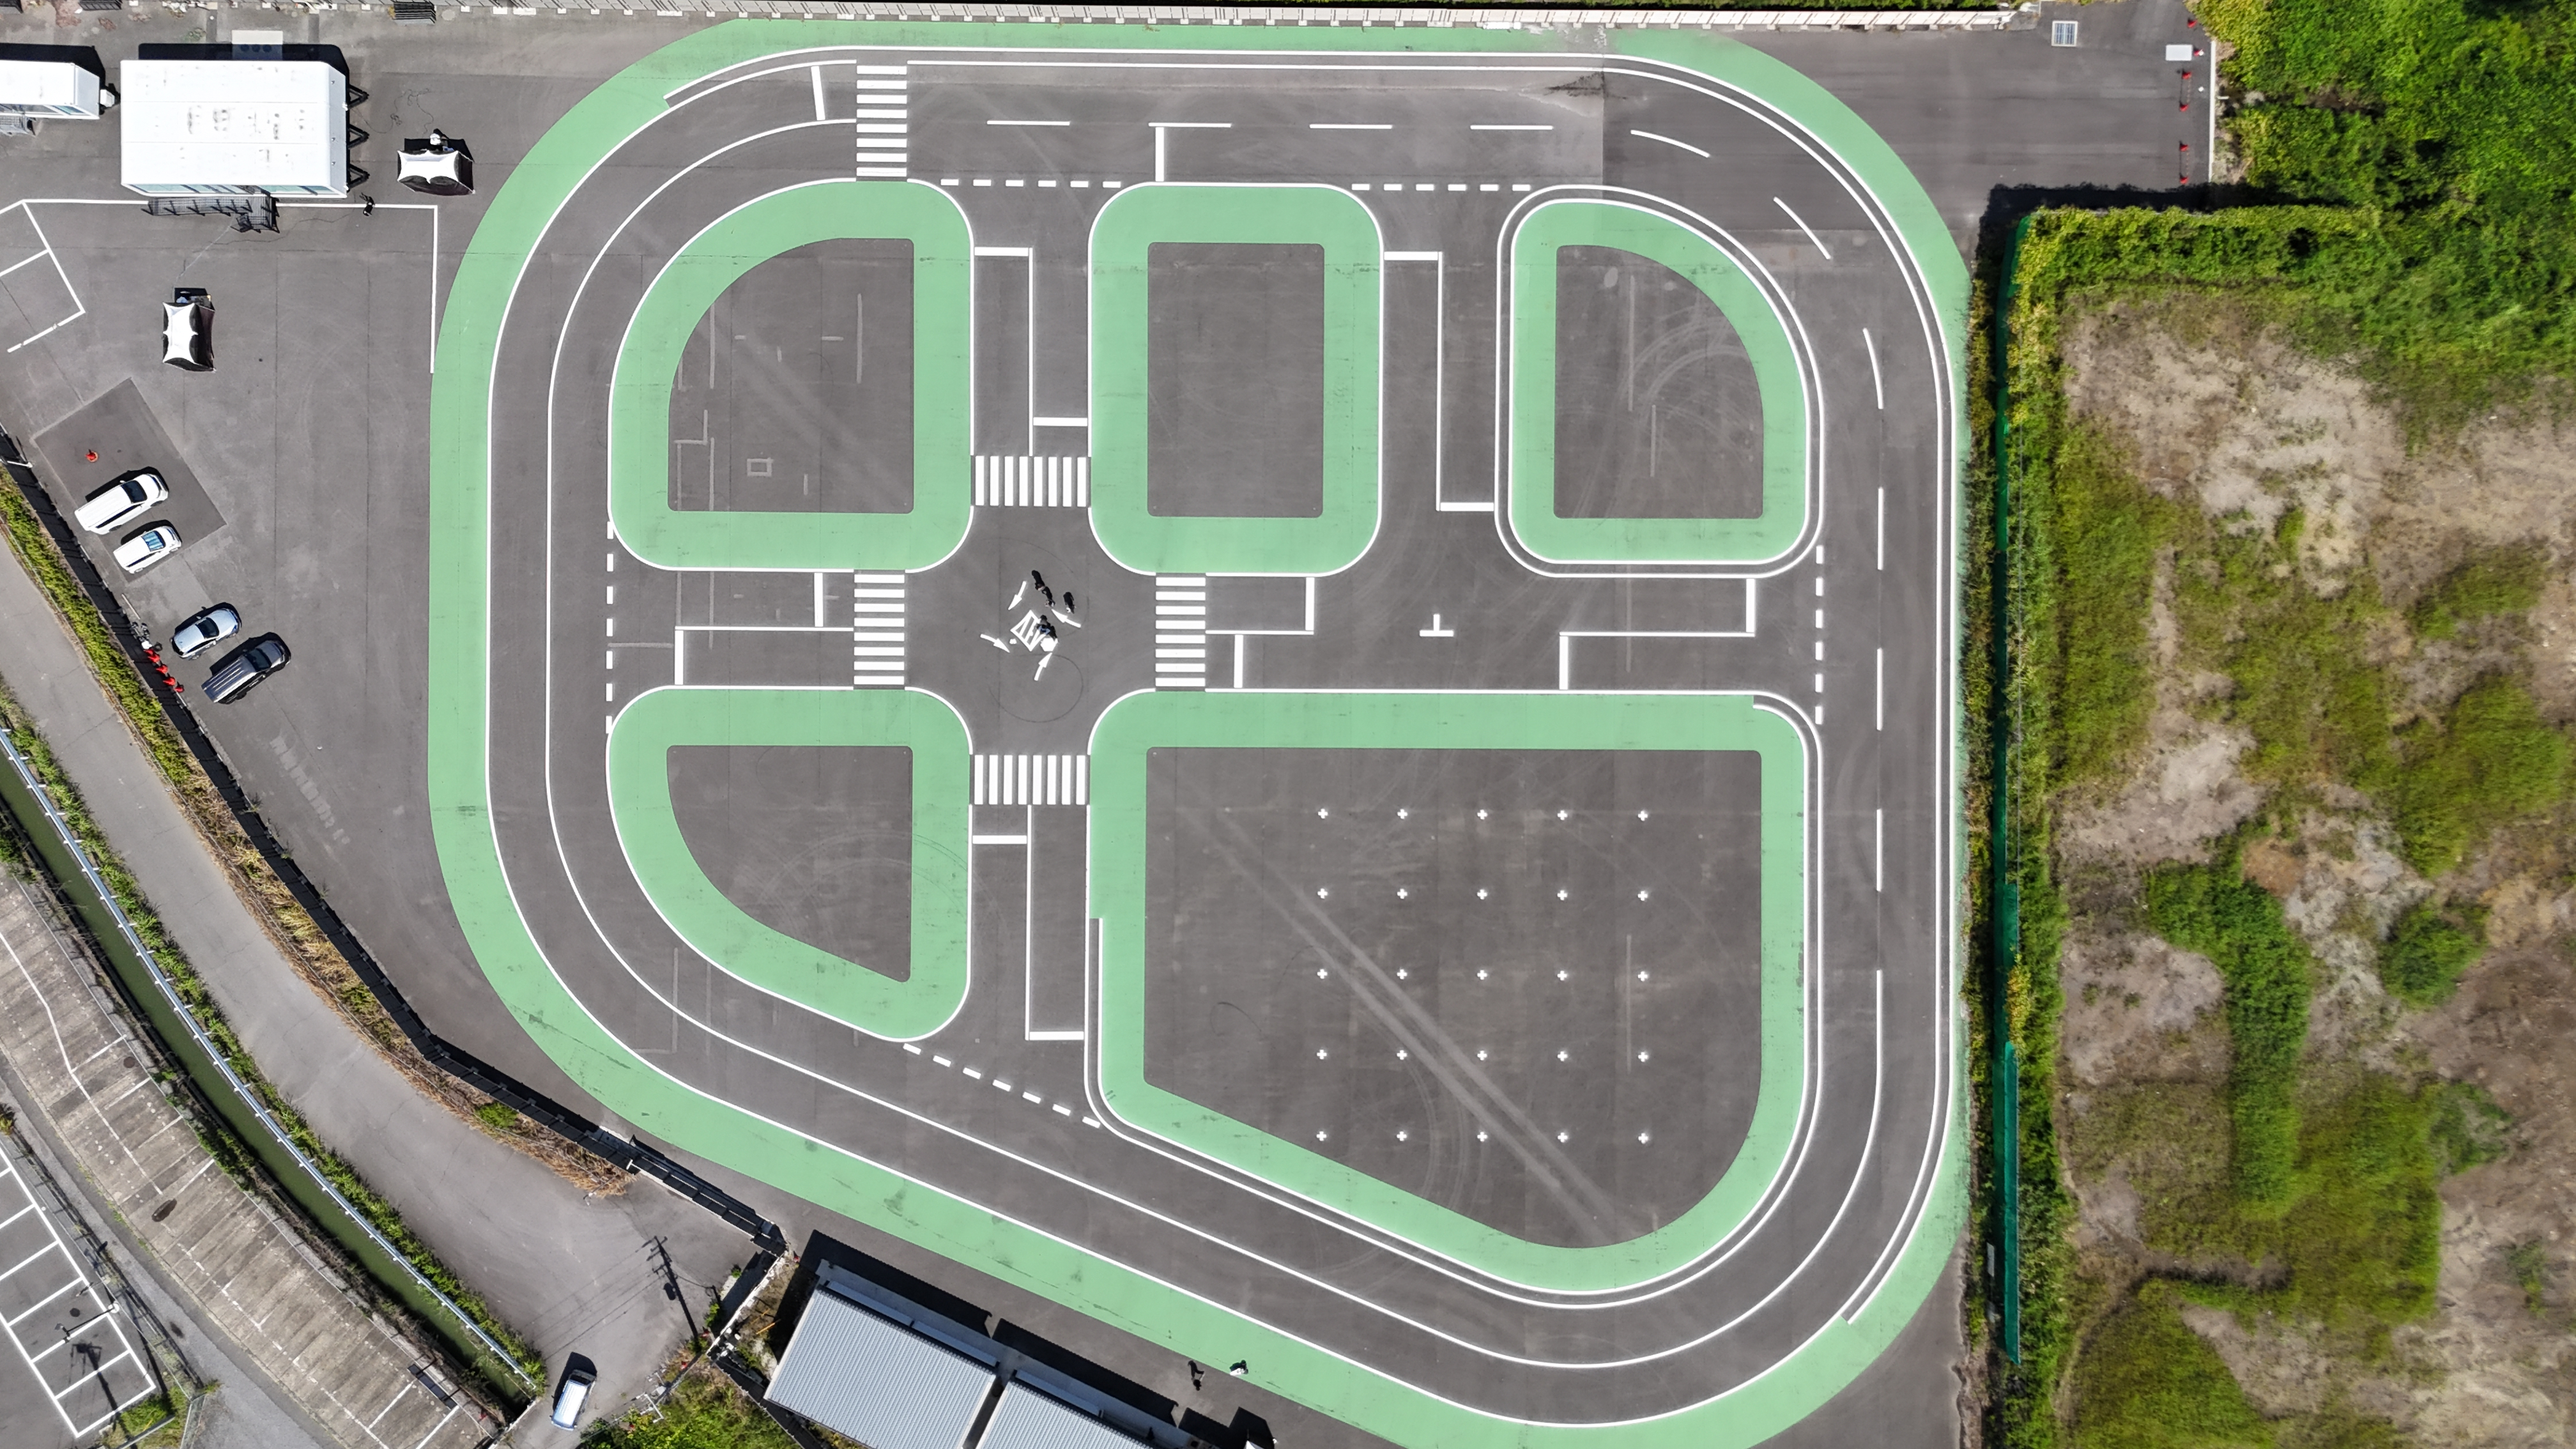
\includegraphics[keepaspectratio, scale=0.1]
      {images/AerialViewAndMobilitysPerspetiveOfTheCourse.png}
 \caption{Aerial view and mobility perspective of the course}
 \label{fig:course}
\end{figure}


\section{目的}
本研究では, 経路追従をするパッケージを開発して評価を行うことで作成した経路追従のパッケージの有効性を実環境で検証することを目的とする.


\section{論文の構成}
本論文は以下のように構成される.
まず, 2章で使用するセンサ構成とシステムの概要を示す.
3章では経路追従する際に使用するアルゴリズムについて述べる.
4章では開発したシステムを用いて経路追従をした際の追従性能の評価をおこなう.
5章では経路追従の実験結果をまとめる.

\newpage

%
\chapter{要素技術}
\chapter{経路追従に用いたアルゴリズム}
\chapter{実験}
\chapter{結論}

%
%% Main Matter
\mainmatter{}
%
\chapter{序論}
\label{chap:introduction}
%
%\input{introduction/preface}
%
%!TEX root = ../thesis.tex

\section{背景}
AIFormulaは計測自動制御学会と自動車技術会が主催し, 本田技術研究所がサポートする次世代の人工知能モビリティの競技会で, 正式な競技会は2025年から始まる.
AIFormulaは今後ますます需要が高まるであろう自動化システムの技術者を育てるという点で効果が見込まれる.
AIFormulaではハードウェアの変更もある程度許容されているが, 現時点での開発はソフトウェアが中心となる.
ハードウェアは経路追従するために必要なパーツが全て揃っているが, ソフトウェアはデバイスを駆動するサンプルプログラムが用意されているのみである.
競技という性質上, 経路追従などのソフトウェアは各チームで開発することが必要となる.
その点で, コースを自動で走行するためにはソフトウェアの開発は必須となる.

\subsection{ハードウェアとルール}
AIFormulaでは詳細なルールは検討中であるとのことで, 2025年2月に開催される予定のプレ大会以降に詳細なルールが決定される予定となっている.
Fig.1に2025年のプレ大会で使用されるロボットを示す.
プレ大会では指定されたコースを3周する時間で競われる.
LiDARなどは使用できないなど, いくつかの制約がある.

\begin{figure}[H]
  \centering
 \includegraphics[keepaspectratio, scale=0.6]
      {images/ExteriorViewOfTheMobilityPlatform.png}
 \caption{Exterior view of the mobility platform}
 \label{fig:robot view}
\end{figure}

\subsection{コース}
Fig.2にAIFormulaのコースを示す.
周囲に高い建造物のない平坦なコースである.


\begin{figure}[H]
  \centering
 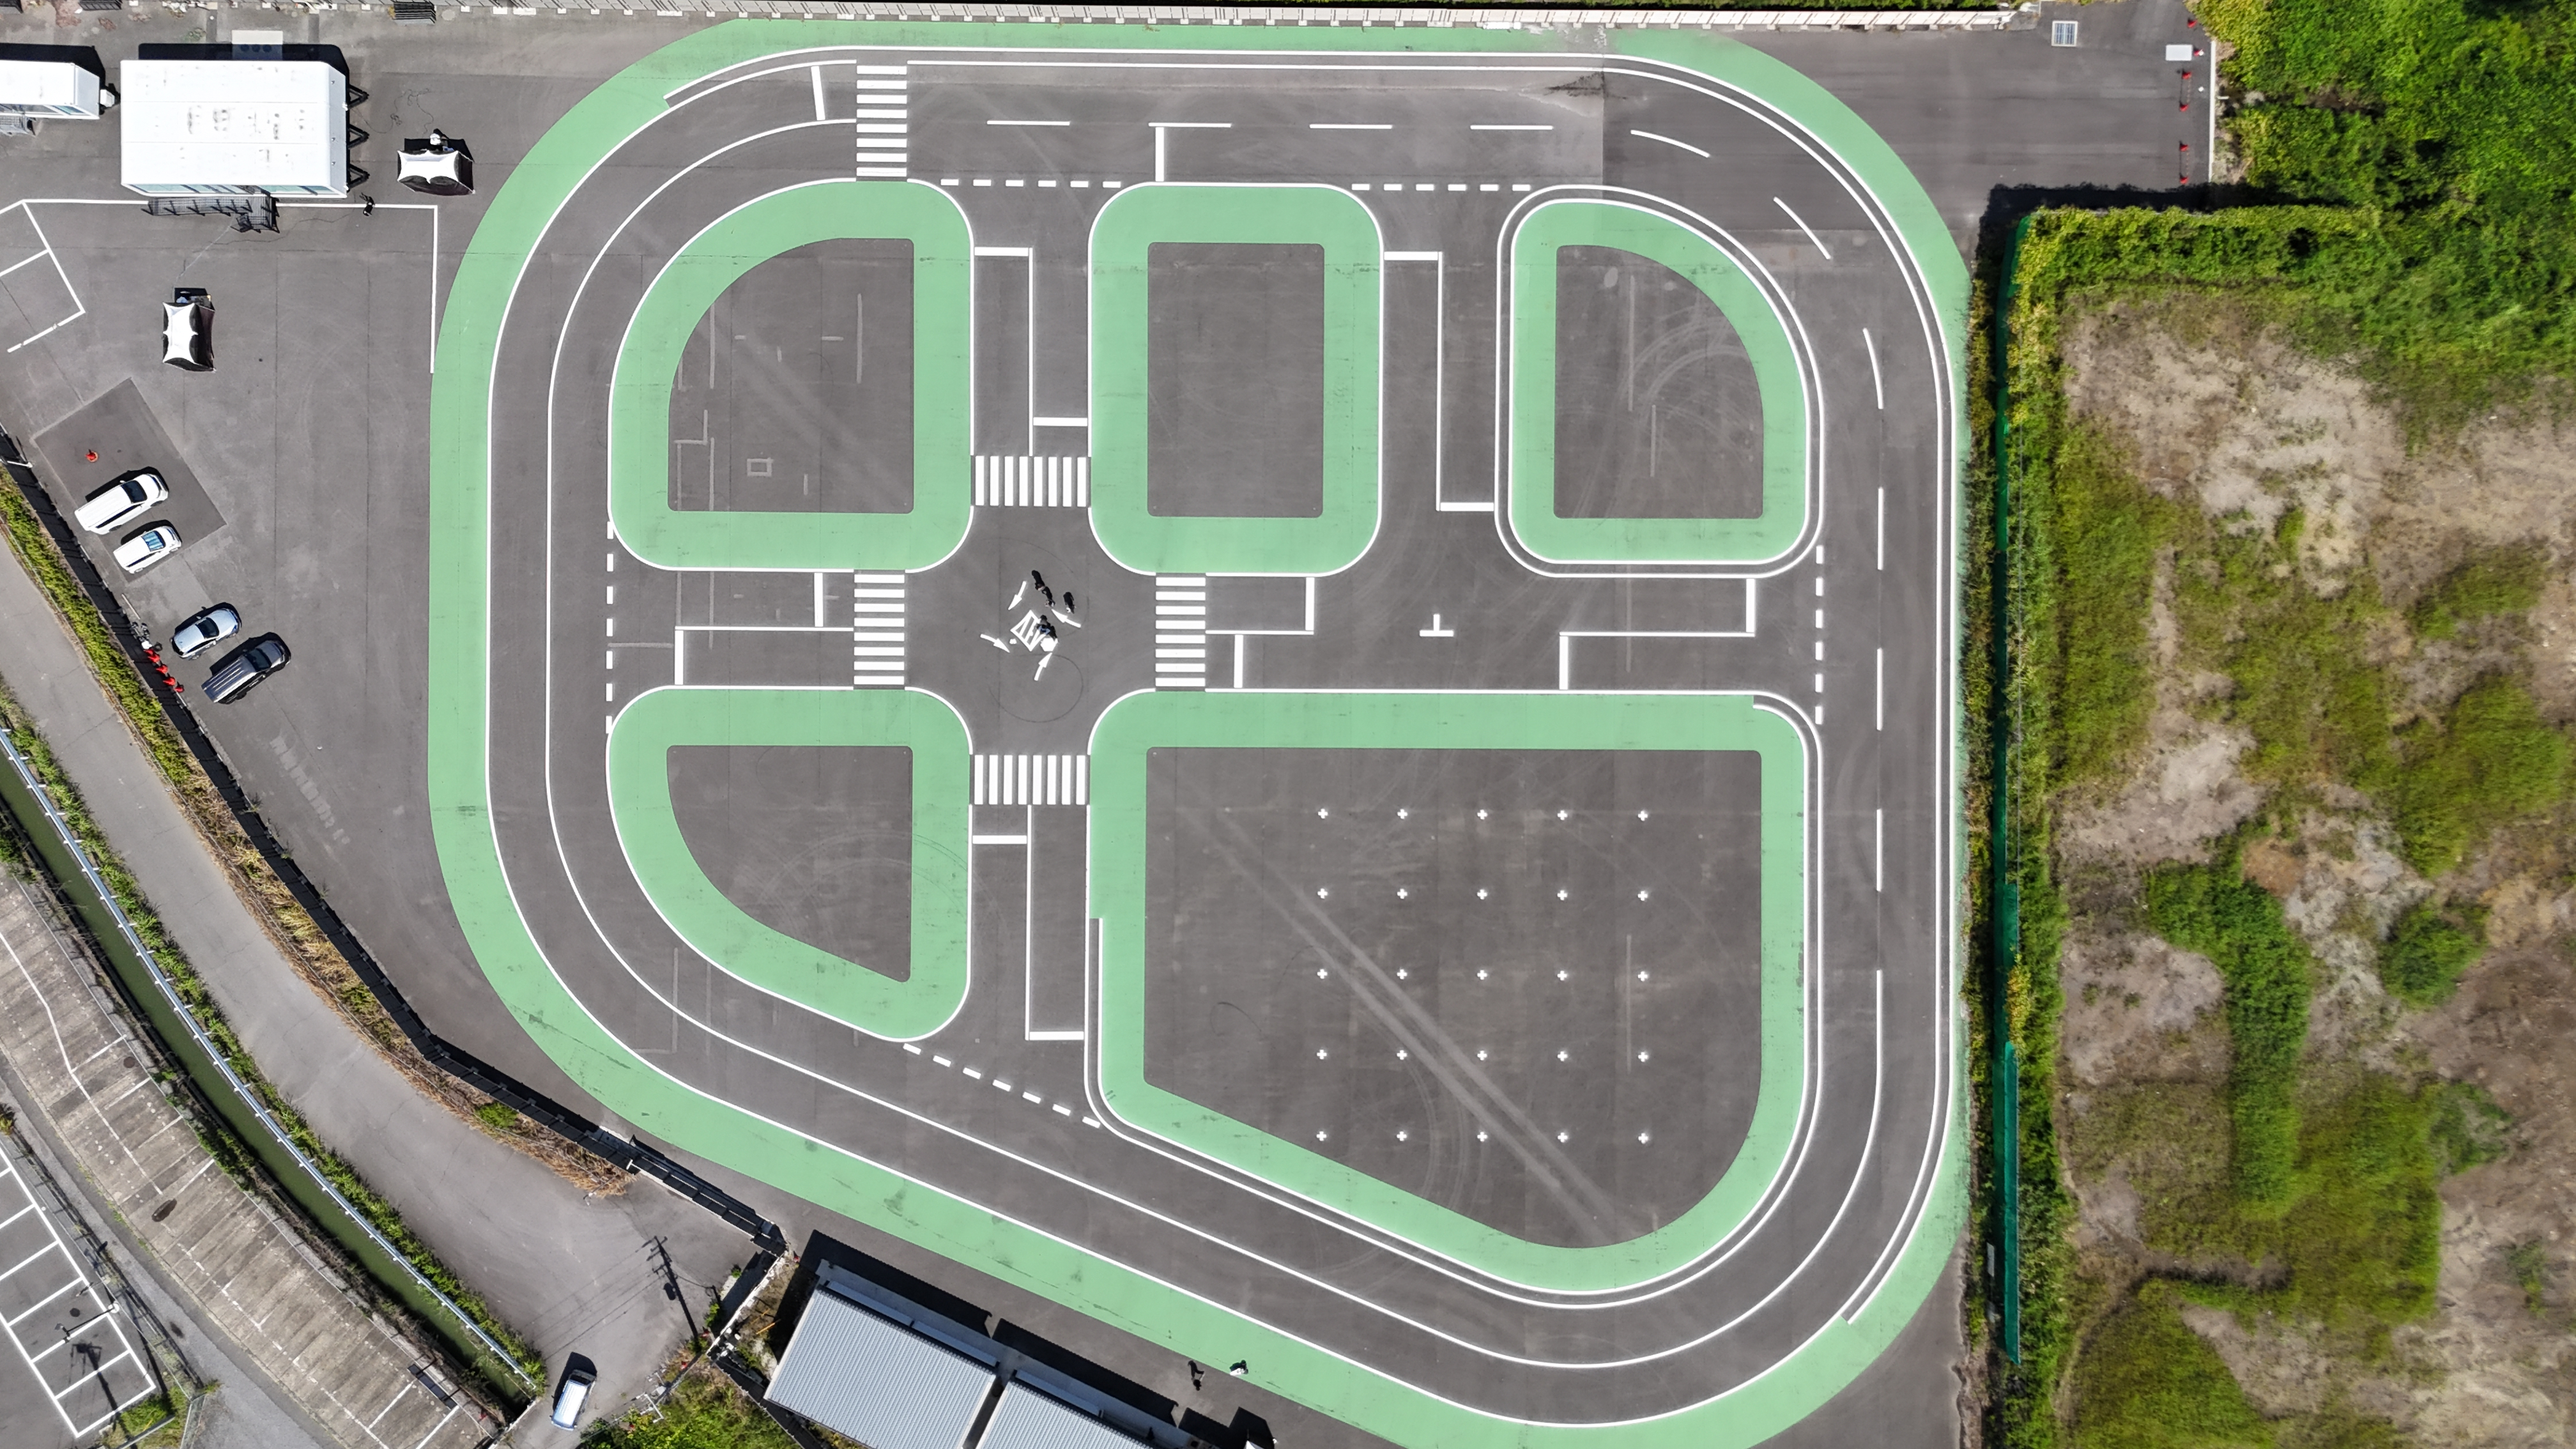
\includegraphics[keepaspectratio, scale=0.1]
      {images/AerialViewAndMobilitysPerspetiveOfTheCourse.png}
 \caption{Aerial view and mobility perspective of the course}
 \label{fig:course}
\end{figure}


\section{目的}
本研究では, 経路追従をするパッケージを開発して評価を行うことで作成した経路追従のパッケージの有効性を実環境で検証することを目的とする.


\section{論文の構成}
本論文は以下のように構成される.
まず, 2章で使用するセンサ構成とシステムの概要を示す.
3章では経路追従する際に使用するアルゴリズムについて述べる.
4章では開発したシステムを用いて経路追従をした際の追従性能の評価をおこなう.
5章では経路追従の実験結果をまとめる.

\newpage

%
\chapter{要素技術}
\chapter{経路追従に用いたアルゴリズム}
\chapter{実験}
\chapter{結論}

%ここにディレクトリのパスを追加していく
%
%% Back Matter
\backmatter{}
%
%!TEX root = ../thesis.tex
% \bibliographystyle{unsrt}
\bibliographystyle{junsrt}
%\bibliography{report}
\nocite{*}
\bibliography{main_bibliography}
%
%!TEX root = ../thesis.tex
\chapter*{付録}

実験動画を Youtubeで公開している.
また, 本研究で開発したパッケージやAIFormula千葉工業大学チームが開発したリポジトリはgithubで公開している.

\begin{itemize}
  \item 実験動画のリンク
    https://youtu.be/nZ-q6UWQDuA
  \item githubのリンク
    https://github.com/open-rdc/aiformula
\end{itemize}

\addcontentsline{toc}{chapter}{付録}

%
%!TEX root = ../thesis.tex
\chapter*{謝辞}
\addcontentsline{toc}{chapter}{謝辞}

本研究を進めるにあたり,1年に渡り, 熱心にご指導を頂いた林原靖男教授に深く感謝いたします.
また, チームの活動を通して知識や技術を教えていただきました, AIFormula千葉工業大学チームの皆様に感謝いたします.
最後に, 日常生活の多くを支えてくださった両親と祖父母に感謝いたします.

%


%

\end{document}
